% !TEX root = ../22830110_dissertation.tex

\chapter{Implementation and Development}
\label{chap:implementation}

\section{Technology Stack}
The \textit{ai\_review\_notes} application is designed as a Flask-based web service capable of rapid asynchronous execution. This modern stack was selected to handle the robust requirements of both data engineering and complex NLP tasks.
\begin{itemize}
    \item \textbf{Backend Framework:} Python, Flask, and Celery are used for handling background task processing and enabling real-time UI event emission.
    \item \textbf{Database Architecture:} The application employs SQLite for rapid local development and Azure SQL for production deployment via ODBC normalization, ensuring scalable data storage.
    \item \textbf{AI Orchestration:} The CrewAI framework is used to structure the agents, orchestrating their interaction with Azure OpenAI API endpoints. The fine-tuned configurations were based on GPT-4.1, while the prompt-engineering baseline used the Azure-hosted \texttt{gpt-5.4} deployment.
    \item \textbf{Data Integration:} The Python Xero SDK is deeply integrated for API connectivity, managing token caching securely.
\end{itemize}

Azure is used here for a governance reason as much as a technical one. The system processes sensitive company financial data, and the Azure-hosted model and storage components provide a more appropriate protection boundary for that material than consumer-facing AI tooling. For that reason, the submitted repository intentionally excludes live \texttt{.env} files and active credentials. The code paths are present, but access to live resources is restricted. A working demonstration remains available on request under supervised conditions.

\begin{figure}[H]
    \centering
    \begin{minipage}{0.12\textwidth}
        \centering
        
\includegraphics[width=\textwidth]{figures/flask_logo}
    \end{minipage}\hfill
    \begin{minipage}{0.12\textwidth}
        \centering
        
\includegraphics[width=\textwidth]{figures/celery}
    \end{minipage}\hfill
    \begin{minipage}{0.12\textwidth}
        \centering
        
\includegraphics[width=\textwidth]{figures/azure_sql_logo}
    \end{minipage}\hfill
    \begin{minipage}{0.12\textwidth}
        \centering
        
\includegraphics[width=\textwidth]{figures/xero_logo}
    \end{minipage}\hfill
    \begin{minipage}{0.12\textwidth}
        \centering
        
\includegraphics[width=\textwidth]{figures/crewai_logo}
    \end{minipage}\hfill
    \begin{minipage}{0.12\textwidth}
        \centering
        
\includegraphics[width=\textwidth]{figures/azure_logo}
    \end{minipage}\hfill
    \begin{minipage}{0.12\textwidth}
        \centering
        
\includegraphics[width=\textwidth]{figures/azure_ai_foundry}
    \end{minipage}
    \caption{Core Technology Stack Components}
    \label{fig:tech_stack_logos}
\end{figure}

\section{Data Acquisition and Processing Pipeline}
The foundation of the system is built upon a robust data acquisition and processing pipeline designed to handle heterogeneous client data formats. 

\subsection{Client Identification and Mapping}
The process initiates with data acquisition from raw Excel ledgers provided by the firm. The system extracts the client name from these files and performs a cross-reference mapping against Xero's internal database to securely identify the corresponding \texttt{contact\_id} and \texttt{tenant\_id}. This dynamic mapping bridges the gap between static spreadsheet reports and live cloud accounting environments.

\subsection{Data Fetching and Organisation}
Once the correct Xero tenant is authenticated via the API, the system automatically fetches the complete transaction history, chart of accounts, and ledger data for the specified financial year. The raw JSON payloads retrieved from Xero are often unstructured and overly verbose. The processing engine steps in to systematically organise this data. It filters out irrelevant metadata and categorises transactions into standard accounting classes (Assets, Liabilities, Equity, Revenue, Expenses).

\subsection{Azure Blob and Xero Re-Enrichment Pipeline}
The dissertation dataset was constructed using a two-stage cloud pipeline. First, historical structured working-paper JSON files were loaded from Azure Blob Storage containers containing PHM, Chris, and other client folders. Each file was transformed into a chat-style JSONL record with three components: a system instruction defining the UK accountant role, a user message containing the Xero trial balance and transaction context, and an assistant message containing the target accountant-written review note. The resulting records were split into training and validation JSONL files before upload to Azure AI Foundry for supervised fine-tuning.

Second, lightweight records containing only metadata were re-enriched directly from the Xero API when a valid \texttt{tenant\_id} and year-end date were available. The Xero OAuth2 refresh-token flow was used to maintain access, after which the pipeline fetched reports and transactions for the relevant two-year period. This design ensured that the model was not trained solely on stale spreadsheet exports: where possible, the trial balance and transaction context were reconstructed from live accounting-system data. The implementation also included a connection-gap analysis, matching company names in blob storage against connected Xero tenants to identify clients requiring additional authorisation.

\begin{figure}[H]
    \centering
    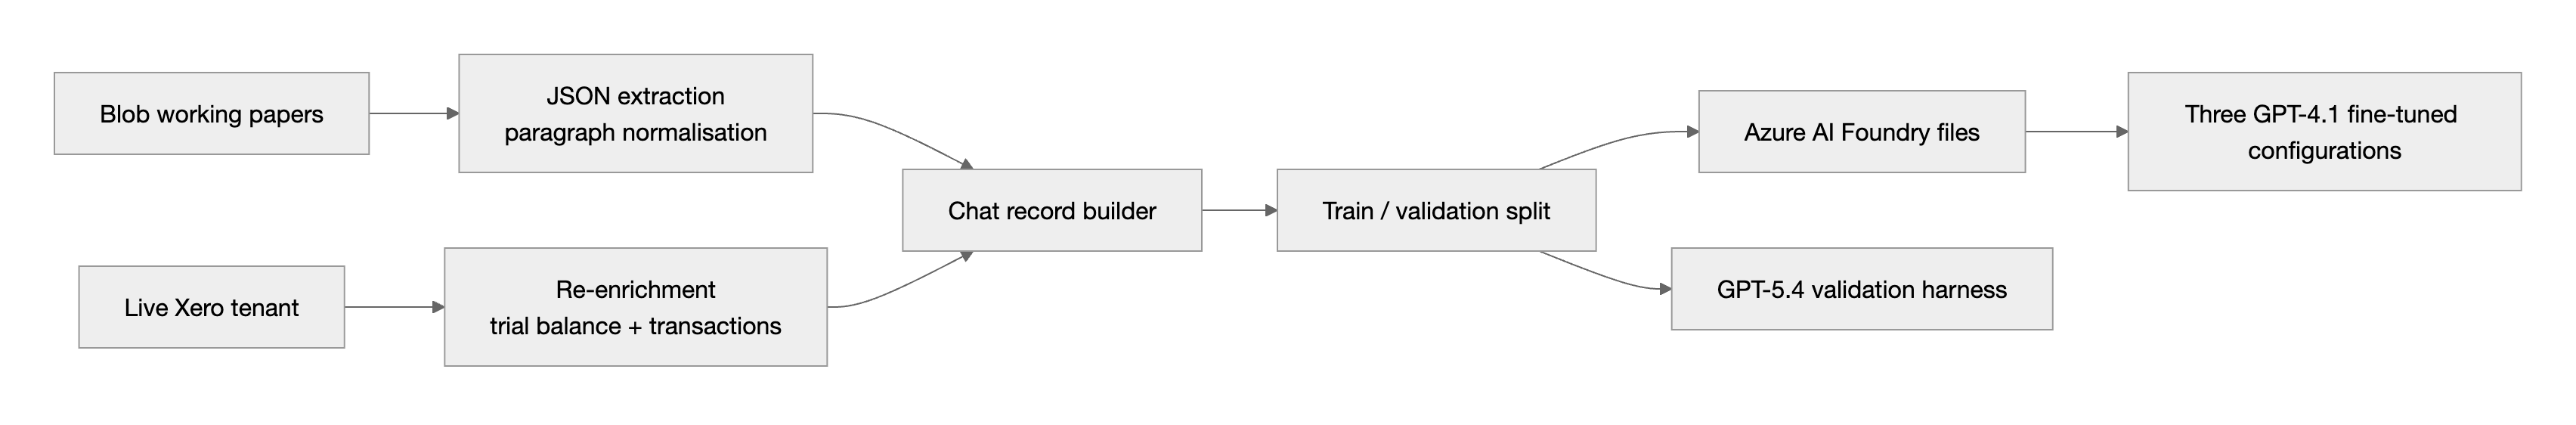
\includegraphics[width=0.92\textwidth]{figures/data_pipeline_lifecycle}
    \caption{Dataset Construction and Validation Lifecycle}
    \label{fig:data_pipeline_lifecycle}
\end{figure}

Figure \ref{fig:data_pipeline_lifecycle} shows the full dataset path. Blob working papers and live Xero re-enrichment feed the same chat-record builder, after which the records are split for fine-tuning and for prompt-engineering validation.

\subsection{Implementation Example: From Raw Balances to a Review Note}
One way to understand the implementation is to follow a real case through the pipeline. One validation example contains large balances for development costs, legal and professional fees, loan interest, investor-related expenditure, and a growing share premium account. At the raw-data level, it appears as a dense trial balance with little narrative structure. The pipeline converts that input into a sequence of machine-usable stages.

First, the ingestion layer preserves the original balances and metadata exactly, without allowing the language model to ``reinterpret'' them numerically. Second, the context builder turns the balance sheet and transaction summaries into a constrained prompt containing the relevant accounting facts. Third, the note-generation harness supplies this context to either a fine-tuned GPT-4.1 model or the GPT-5.4 prompt baseline. The output is not judged only on fluency. It must also preserve the control issue in the source material: further share issue documentation is still required before the final equity position can be treated as complete.

A less constrained prototype could generate a plausible paragraph about investment growth while inventing certainty around shareholdings or paperwork status. The implemented pipeline instead follows the working-paper approach used by the accountants: where the evidence is incomplete, the output should say so directly. That behaviour can be seen in the redacted examples included later in the dissertation.

\subsection{Deterministic Processing and the Decimal Mandate}
Following organisation, the data undergoes deterministic mathematical processing. The system aggregates journal lines and computes variances against prior periods. In strict adherence to the "Decimal Mandate," all calculations are performed using exact decimal arithmetic. The system automatically identifies "material drivers"—variances exceeding the 10\% threshold—and prepares structured summaries, completely isolating the LLM from any mathematical reasoning.

This design matters most in cases involving directors' loan accounts, payroll, or tax liabilities, where even a one-digit drift can change the meaning of the note. For example, a validation case involving overdrawn director balances requires the narrative to preserve the size and reason for the drawings, while distinguishing them from mileage adjustments and dividends. In such a case, letting the model ``do the maths in language'' would add avoidable risk. The implementation therefore treats the LLM as a constrained narrator of pre-computed accounting facts.

\section{Fine-Tuning and Test Environment Construction}
To adapt the general-purpose LLMs to the specific stylistic constraints and reporting formats of PHM UK, an extensive fine-tuning and testing environment was constructed.

\subsection{Model Fine-Tuning}
Historical accounting notes and their corresponding data sets were compiled to create a high-quality training corpus. The system fine-tuned multiple iterations of state-of-the-art models on varying data formats to ensure they internalised the firm's strict "You" persona and paragraph structuring rules. This fine-tuning drastically improved the models' ability to synthesise the deterministic JSON data into professional, audit-ready narrative without hallucination.

\subsection{Test Environment}
The \texttt{experiments/} module serves as a local test environment. It isolates the scoring mechanisms and model benchmarking protocols from the main web application. The final live benchmark harness (\path{experiments/benchmark_dissertation_methods.py}) automates the execution of zero-shot, single-shot, and few-shot prompts against the \texttt{gpt-5.4} Azure deployment and all four callable GPT-4.1 fine-tuned deployments discovered in the Foundry project, tracking numeric fidelity, token usage, and execution time. The harness reads credentials from environment variables only and writes model outputs to a local CSV for later scoring, avoiding the storage of secrets in source code or dissertation artefacts. This is why the submitted repository includes the benchmark code but not the live environment configuration itself.

This test environment was used to check more than readable prose. It was used on cases that appear in real firm workpapers: compliance-related spend described under staff training, legal fees added back for corporation tax, unresolved equity paperwork, and commentary around directors' drawings.

\section{Core Modules and Directory Structure}
The system's logic is modularised to maintain the separation of concerns, dividing the deterministic rules from the stochastic AI generation:
\begin{itemize}
    \item \textbf{App \& Routing (\texttt{app.py}):} The entry point defining the web routes and integrating the CrewAI kickoff process.
    \item \textbf{Agent Definitions (\texttt{agents/crew\_manager.py}):} This file defines the roles, backstories, and goals for the three primary agents: the Financial Analyst, the Writer, and the Reviewer.
    \item \textbf{Data Processing (\texttt{helpers/}):} Contains the Xero API parsers, data masking utilities, and deterministic mathematical rules enforcing the Decimal Mandate.
    \item \textbf{Experiments (\texttt{experiments/}):} A dedicated module for LLM benchmarking and scoring.
\end{itemize}

\section{Provenance and Traceability Implementation}
A core requirement for any accounting software is auditability. To achieve this, every numeric output generated by the system includes either a \texttt{source\_journal\_id} or a \texttt{ledger\_account\_code}. The system automatically generates a \texttt{generation\_log.json} for each session. This log acts as a comprehensive audit trail that snapshots model parameters, prompt templates, and raw input data, ensuring the system remains ``Explainable by Design'' at all times.

\begin{figure}[H]
    \centering
    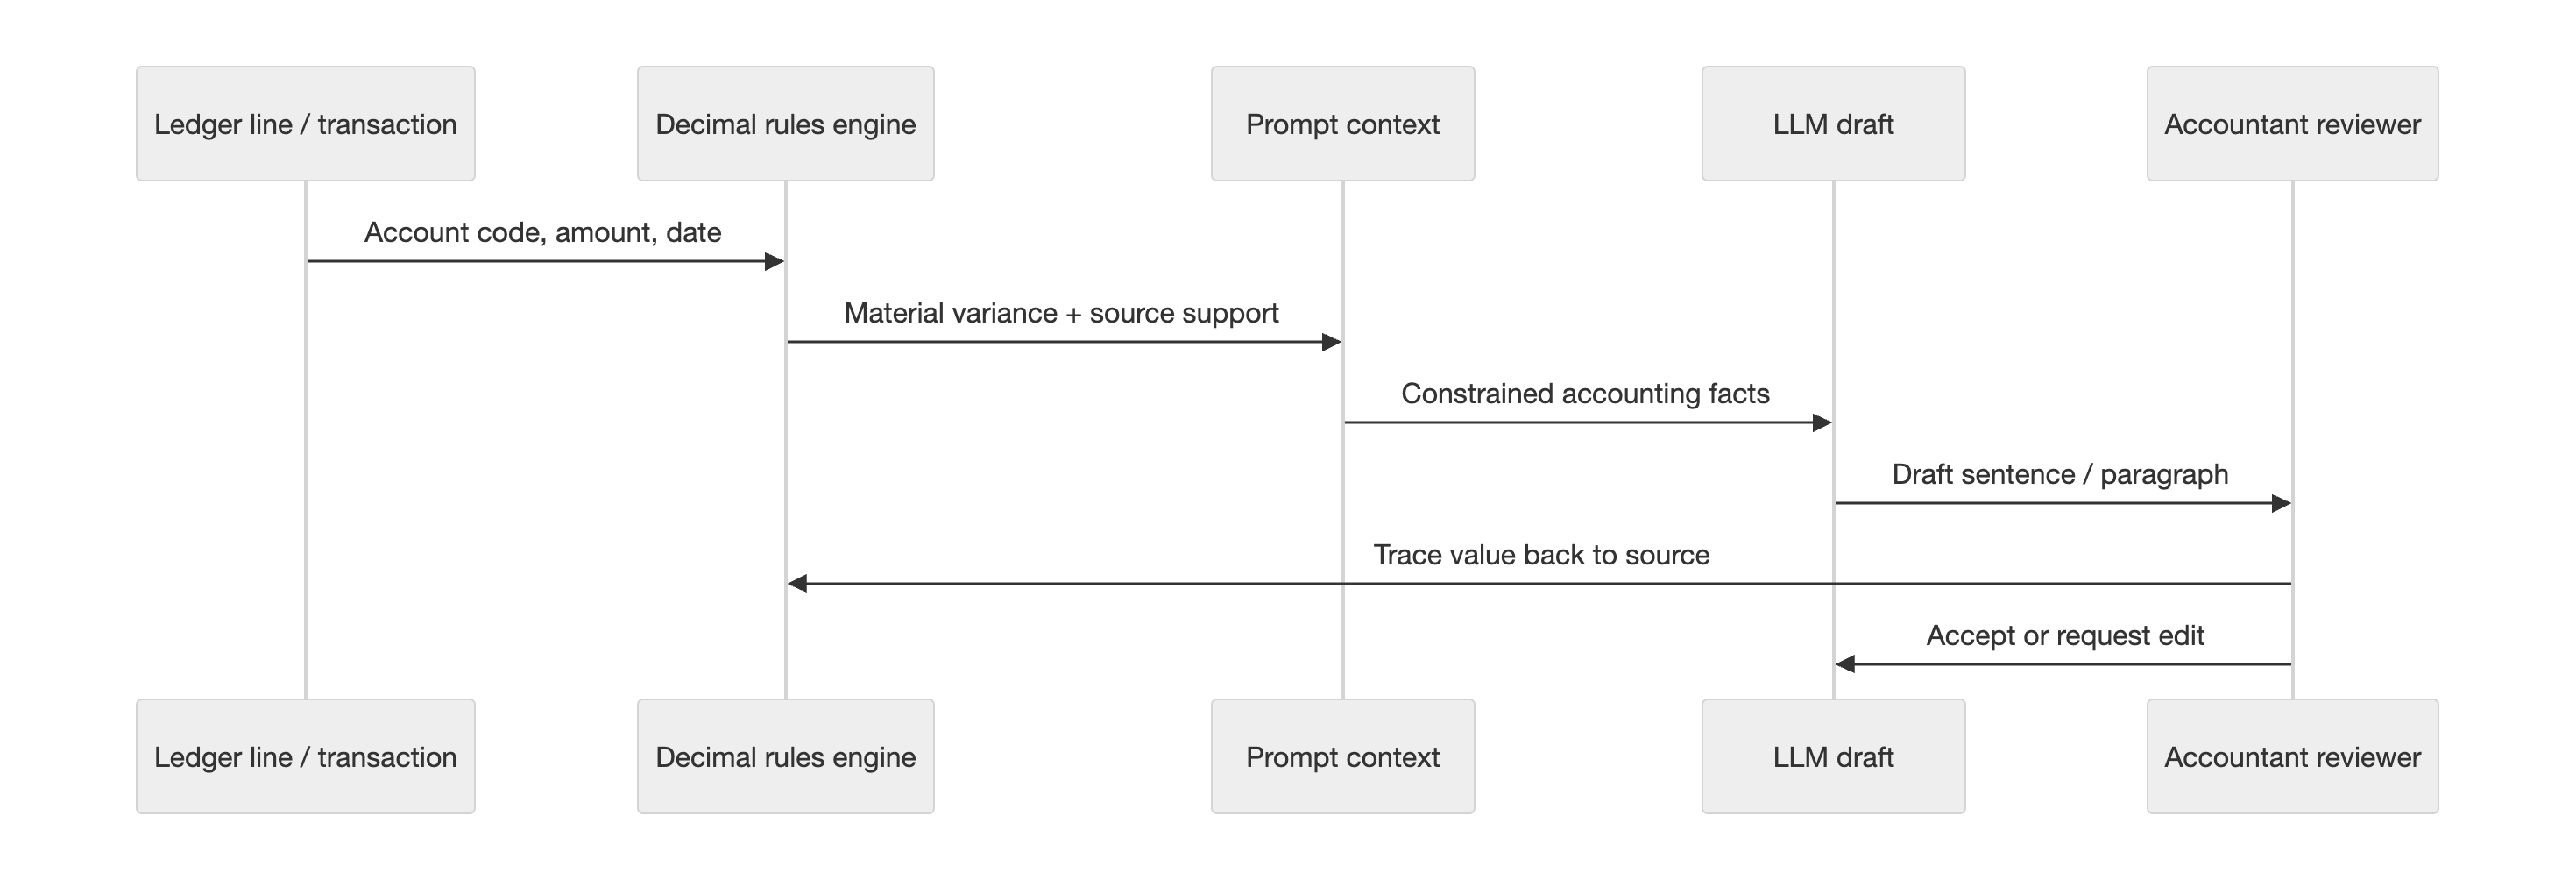
\includegraphics[width=0.88\textwidth]{figures/provenance_trace}
    \caption{Trace from Ledger Evidence to Reviewer Verification}
    \label{fig:provenance_trace}
\end{figure}

Figure \ref{fig:provenance_trace} reduces provenance to the steps that matter during review. A transaction or ledger line is carried through the deterministic engine into the prompt context, then into the draft note, and can be checked again by the reviewer when a figure or claim needs support.

\section{UI/UX Technical Implementation}
The front-end of the application was implemented using Flask's Jinja2 templating engine combined with modern CSS Grid and Flexbox layouts. The primary design goal was to translate the "Accountant Workbench" wireframes into a functional, high-performance interface.

\subsection{Side-by-Side Review Interface}
The main UI component is the \textit{Review Panel}, implemented as a split-view layout. The left pane dynamically renders the deterministic financial data stored in the application's database, while the right pane contains a rich text editor (or styled \texttt{textarea}) for the AI's narrative output. This arrangement lets the user verify the AI's assertions against the raw ledger without moving between screens.

\subsection{Real-time Feedback and Event Handling}
To provide a responsive user experience during the computationally expensive CrewAI execution (which can take 30--60 seconds), the system utilizes asynchronous event emission. As agents complete their sub-tasks—such as "Data Extraction" or "Drafting"—real-time status updates are sent to the UI. This prevents the user from perceiving the system as "frozen" and provides immediate visibility into the multi-agentic reasoning process.

\subsection{Design Consistency and Styling}
Styling was managed through a modular CSS architecture, following the brand's primary colour codes and typography specifications. By avoiding heavy third-party CSS frameworks, the application maintains a lightweight footprint and preserves alignment in dense financial tables.
